
\documentclass[tikz,border=5]{standalone}
\usepackage{tikz}
\usetikzlibrary{calc}
\usepackage{amsmath}
\usepackage{amssymb}

\begin{document}

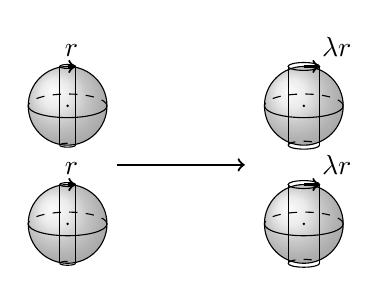
\begin{tikzpicture}[scale=.5]
%draw outline/perimeter of circle 
\shade[ball color = gray!40, opacity = 0.5] (1,2) circle (1cm);
\draw (1,2) circle (1cm);
% XY plane, starting at -2,0  
\draw (0,2) arc (180:360: 1 and 0.3);
% dashed line
\draw[dashed] (2,2) arc (0:180:1 and 0.3);
%node in middle
\fill[fill=black] (1,2) circle (1pt);
%CYLINDER
%vertical lines down
\draw[->,thick] (1,3) -- node[above]{$r$} (1.2,3);
\draw (0.8,3) -- (0.8,1);
\draw (1.2,3) -- (1.2,1);
%top cylinder: ellipse
\draw (1,3) ellipse (0.2 and 0.05);
\draw (0.8,1) arc (180:360:0.2 and 0.05);
\draw [dashed] (0.8,1) arc (180:360: 0.2 and -0.05);


%2ND PLOT
%SPHERE
%draw outline/perimeter of circle 
\shade [yshift=3cm][ball color = gray!40, opacity = 0.5] (1,2) circle (1cm);
\draw [yshift=3cm](1,2) circle (1cm);
% XY plane, starting at -2,0  
\draw [yshift=3cm](0,2) arc (180:360: 1 and 0.3);
% dashed line
\draw[yshift=3cm][dashed] (2,2) arc (0:180:1 and 0.3);
%node in middle
\fill[yshift=3cm][fill=black] (1,2) circle (1pt);
\draw [yshift=3cm] [->,thick] (1,3) -- node[above]{$r$} (1.2,3);
\draw [yshift=3cm](0.8,3) -- (0.8,1);
\draw [yshift=3cm](1.2,3) -- (1.2,1);
%top cylinder: ellipse
\draw [yshift=3cm](1,3) ellipse (0.2 and 0.05);
\draw [yshift=3cm](0.8,1) arc (180:360:0.2 and 0.05);
\draw [yshift=3cm][dashed] (0.8,1) arc (180:360: 0.2 and -0.05);


%ARROW 
\draw[->, thick] (2.25,3.5) -- (5.5,3.5);

%3RD PLOT
%SPHERE
%draw outline/perimeter of circle 
\shade [xshift=6cm,yshift=3cm][ball color = gray!40, opacity = 0.5] (1,2) circle (1cm);
\draw [xshift=6cm,yshift=3cm](1,2) circle (1cm);
% XY plane, starting at -2,0  
\draw [xshift=6cm,yshift=3cm] (0,2) arc (180:360: 1 and 0.3);
% dashed line
\draw [xshift=6cm,yshift=3cm] [dashed] (2,2) arc (0:180:1 and 0.3);
%node in middle
\fill [xshift=6cm,yshift=3cm] [fill=black] (1,2) circle (1pt);
%CYLINDER
\draw [xshift=6cm,yshift=3cm] [->,thick] (1,3) -- node[above right]{$\lambda r$} (1.4,3);
\draw [xshift=6cm,yshift=3cm](0.6,3) -- (0.6,1);
\draw [xshift=6cm,yshift=3cm](1.4,3) -- (1.4,1);
%top cylinder: ellipse
\draw [xshift=6cm,yshift=3cm](1,3) ellipse (0.4 and 0.1);
\draw [xshift=6cm,yshift=3cm](0.6,1) arc (180:360:0.4 and 0.1);
\draw [xshift=6cm,yshift=3cm][dashed] (0.6,1) arc (180:360: 0.4 and -0.1);


%4RD PLOT
%SPHERE
%draw outline/perimeter of circle 
\shade [xshift=6cm][ball color = gray!40, opacity = 0.5] (1,2) circle (1cm);
\draw [xshift=6cm](1,2) circle (1cm);
% XY plane, starting at -2,0  
\draw [xshift=6cm](0,2) arc (180:360: 1 and 0.3);
% dashed line
\draw [xshift=6cm][dashed] (2,2) arc (0:180:1 and 0.3);
%node in middle
\fill [xshift=6cm][fill=black] (1,2) circle (1pt);
%CYLINDER 
\draw [xshift=6cm] [->,thick] (1,3) -- node[above right]{$\lambda r$} (1.4,3);
\draw [xshift=6cm](0.6,3) -- (0.6,1);
\draw [xshift=6cm](1.4,3) -- (1.4,1);
%top cylinder: ellipse
\draw [xshift=6cm](1,3) ellipse (0.4 and 0.1);
\draw [xshift=6cm](0.6,1) arc (180:360:0.4 and 0.1);
\draw [xshift=6cm][dashed] (0.6,1) arc (180:360: 0.4 and -0.1);

\end{tikzpicture}

\end{document}